\section{Results}
\label{sec:results}
\input table_epsilon
We evaluate TRANSIT on each of our
input maps and measure its performance in terms of:
number of transit nodes per cell (T), database size (DB)
and global query time.
To provide a common point of reference we report the latter
in terms of \emph{speedup} which we define
as relative improvement vs. standard A* search. The exception is Table~\ref{table:epsilon}
where we report times in $\mu$s.
Database size is always in MB.

\subsection{Symmetry Reduction}
In Table \ref{table:epsilon} we give results
for our $\epsilon$-based symmetry breaking approach.
We run TRANSIT on two variants of each input map:
one where diagonal transitions are allowed
and the other where they are not. Both are common in
games and often studied in the literature.

In the case where diagonal transitions are disallowed the
addition of random $\epsilon$-costs to edge-weights has a dramatic
effect, reducing the number of identified transit nodes by a
factor of between 2-4 and reducing global query times by anywhere
between 2.5 times to over one order of magnitude.
When diagonal transitions are allowed (which is always the case
in the remainder of this section)
the improvement is less dramatic but remains strongly positive:
we reduce the number of transit nodes by between 10-25\%
and improve global query times by up to a factor of 2.

\subsection{Comparative Performance}
\label{sec:results}

\begin{figure*}[tb]
   \begin{center}
	   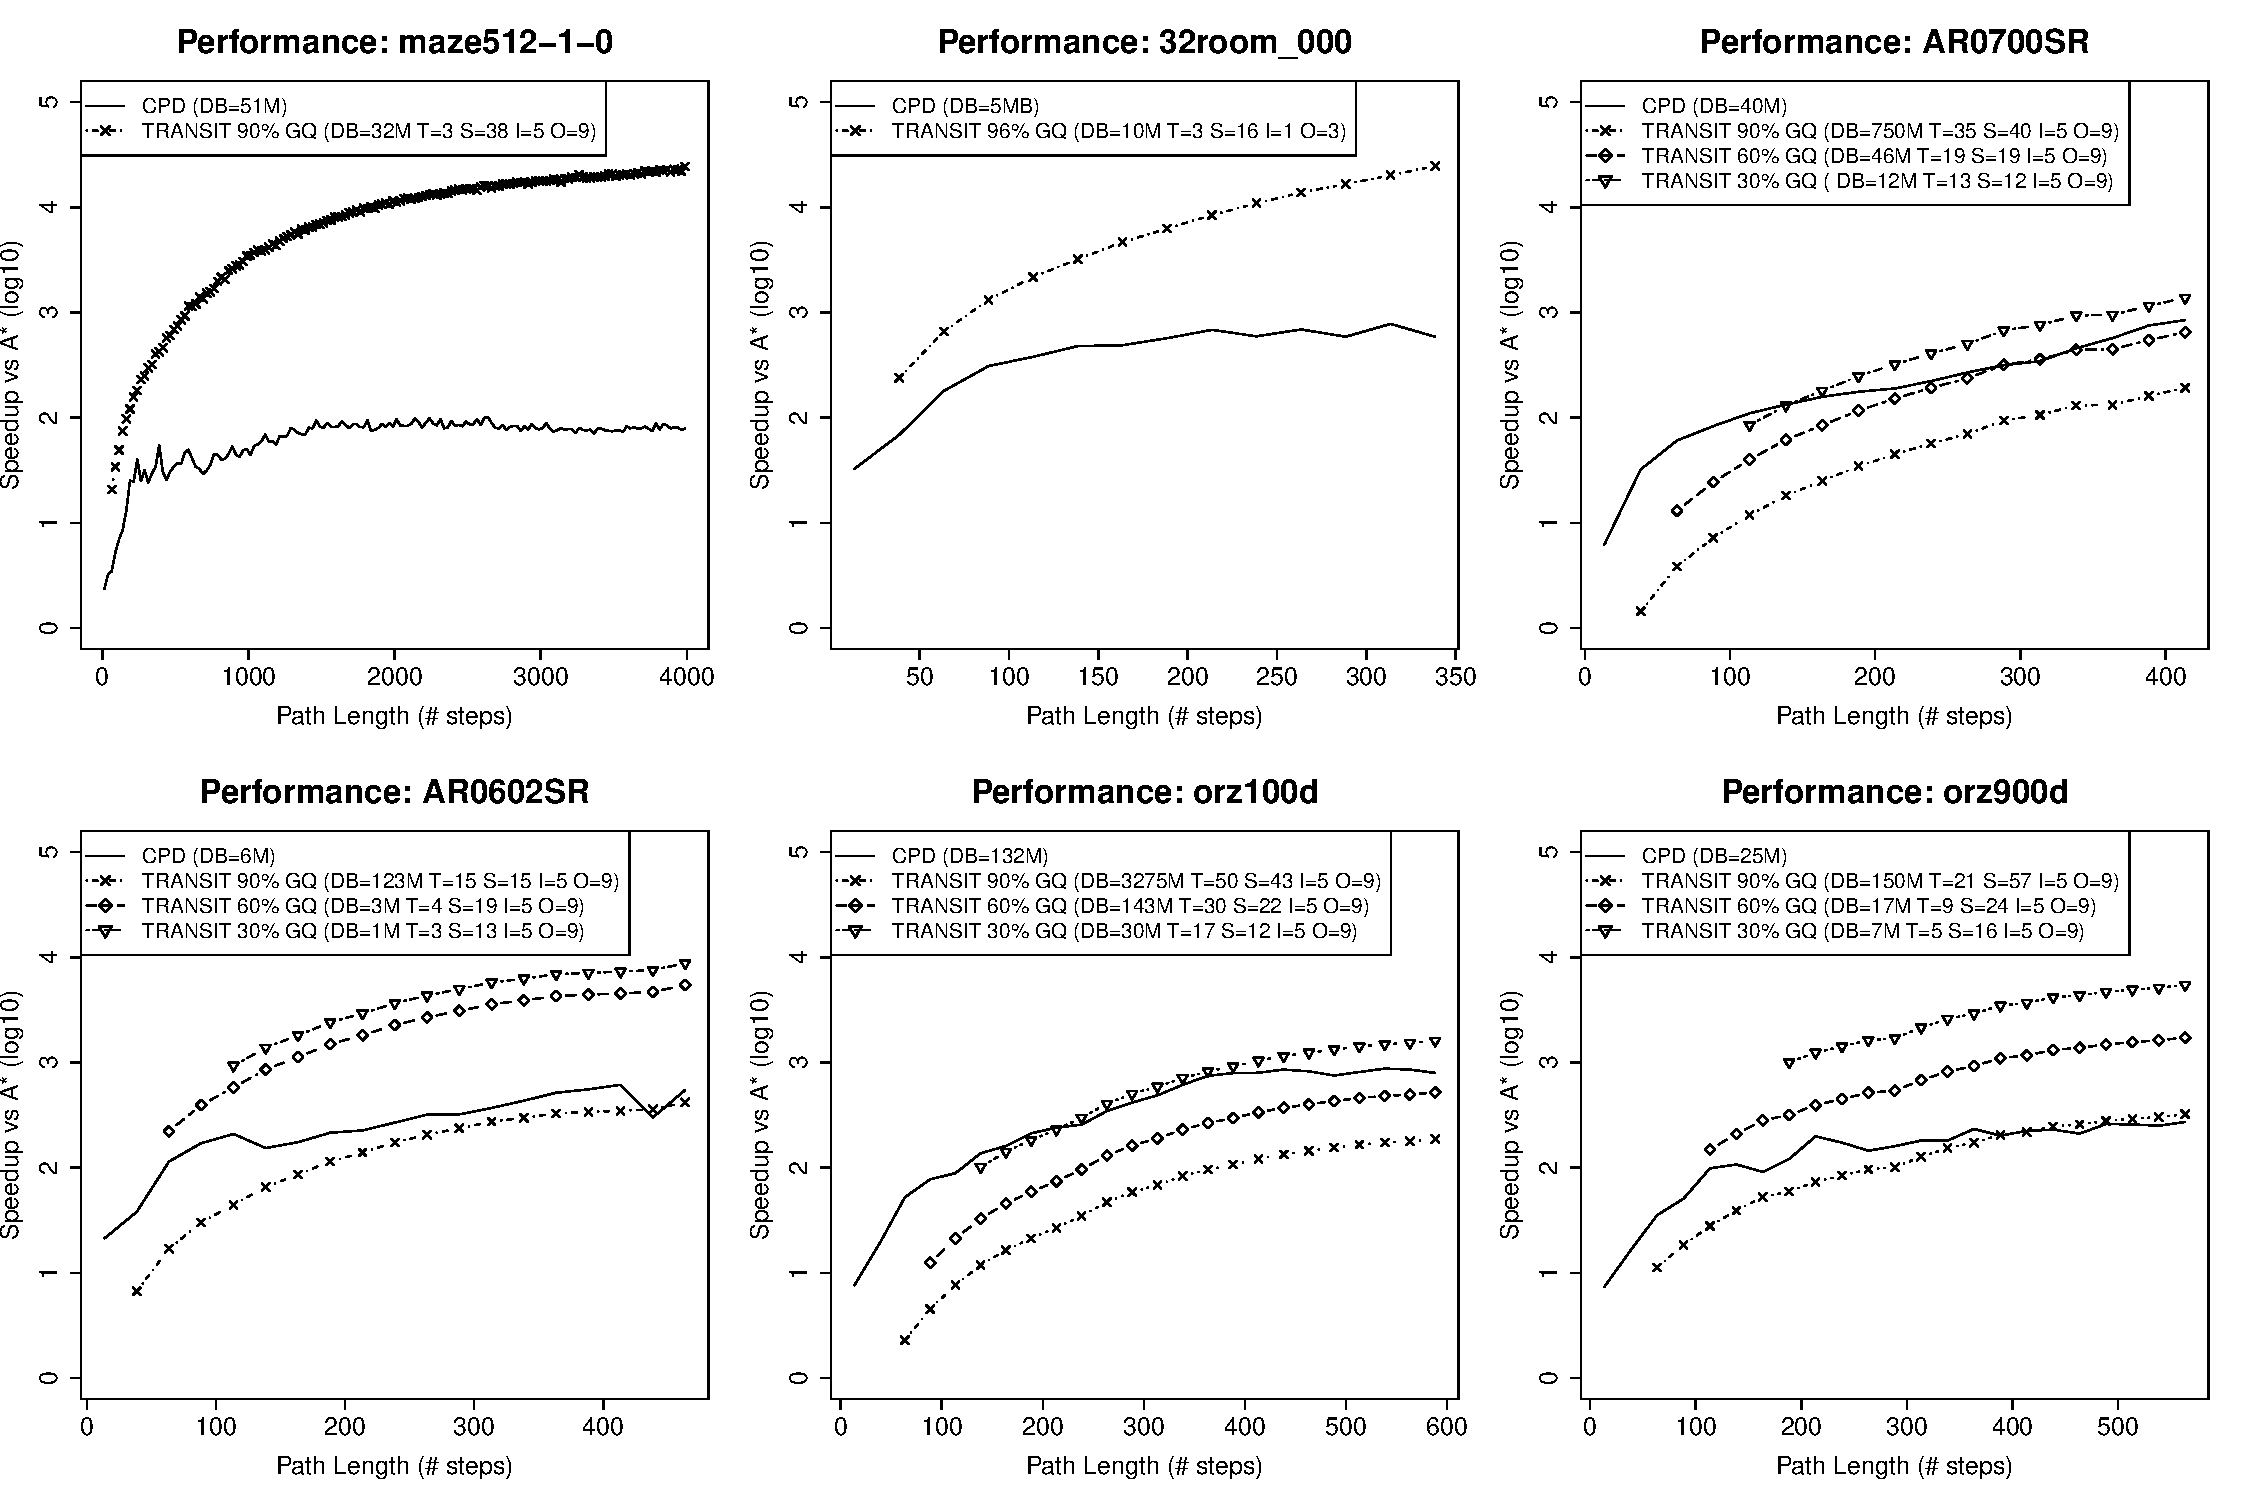
\includegraphics[width=2.0\columnwidth, trim = 10mm 10mm 10mm 0mm]
		{diagrams/speedup.pdf}
   \end{center}
   \caption{Search time speedup (i.e. relative improvement) of TRANSIT and CPDs vs. A*. Note the log10 scale on the y-axis.}
\label{fig:speedup}
\end{figure*}

We compare TRANSIT with Compressed Path Databases ~\cite{botea11}
on each map in our test set~\footnote{NB: diagonals are always allowed here.}.
CPDs are a new and highly effective procedure for compressing
all-pairs data. As is often the case with TRANSIT, CPDs can solve
distance queries optimally with no state-space search. Only a linear
number of lookups into a compact database are required
(the number is equal to the individual steps on the path).
By comparison TRANSIT performs a single lookup operation which 
compares a up to a quadractic number of local transit nodes.
Figure \ref{fig:speedup} summarises our findings.
 Note that values along the y-axis are log10.

We plot in most cases three curves for TRANSIT; each one represents
a different set of preprocessing parameters including different abstract
grid size (S) and different sizes for the Inner square $I$
and Outer square $O$ (we measure both of these in terms of
cells in the abstract grid). We also give the average number of
transit nodes (T) for each cell in the abstract graph and the percentage of
queries which are global (GQ) and do not require any state-space search.
Remaining local queries are omitted (these paths are usually short and can be
solved using any available search algorithm; for example Jump Point
Search~\cite{harabor11b}).

We observe that on domains containing no symmetries (Mazes) or only
short symmetric path segments (Rooms) TRANSIT outperforms
CPDs by between one and two orders of magnitude (and up to 4 orders
improvement over A* search). TRANSIT requires a moderate amount of
storage (32MB and 10MB respectively) and covers 90\% of all queries without search
(the remaining 10\% are local). CPDs require 51MB and 5MB respectively
and cover all queries. Notice that we store only a very small number
of transit nodes per cell. We experimented with different preprocessing
parameters beyond those given in Figure~\ref{fig:speedup} but were unable
to reduce this number further for additional speed gains.

The remaining domains, particularly orz100d and AR0700SR, are characterised
by large open areas and long symmetric path segments that often
span several cells in the abstract grid. These symmeries
are not pruned effectively by TRANSIT using $\epsilon$-costs.
As a consequence, for 90\% coverage, its performance is dominated by CPDs;
both in terms of time and database size.
We ran additional experiments on these problems using two smaller values
for global query coverage: 60\% and 30\%. We used a coarser abstract
grid in these cases, having larger (absolute) values for $I$ and
$O$. 60\% global query coverage omits all paths of lengths
between 50-125 (depending on the domain). 30\% coverage can omit in some
cases all paths up to length 175.
In return for this tradeoff, we see a dramatic reduction in the 
average number of access nodes per cell (T) and a corresponding
improvement in performance: TRANSIT is shown to be up to an order of
magnitude faster than CPDs using 30\% global query coverage and requires
substantially less memory; in some cases just a few MB.
For 60\% global query coverage, TRANSIT is comparable with CPDs, both
in terms of peformance and database size.

\subsection{Discussion}
We have shown that TRANSIT is able to compete with and even outperform CPDs for a certain
class of distance query: those where the start and goal are not in close proximity.
Such problems are usually considered difficult for state-space search algorithms but also for CPDs because
more lookups are required and each lookup has an associated, and often linear-time, cost.
On one hand, CPDs are attractive because they perform well in practice and offer complete
coverage of all queries without resorting to any localized state-space search (as is sometimes
 the case for TRANSIT), as well naturally produce an actual path. On the other hand, CPDs have very long
 preprocessing times and, unlike recent variants of TRANSIT~\cite{verolog2012}, cannot incrementally repair 
the path database in the event of changes to the underlying network.

We find that the two methods have quite different strengths and characteristics and believe them to be
orthogonal and easily combined.
For example: compute a small TRANSIT database covering queries longer than some minimum length.
To cover all remaining queries compute a CPD that contains only paths of lengths less than this minimum: i.e.
during the all-pairs shortest path computation, do not generate any successors beyond the predefined limit.
This is a much smaller subset of nodes than CPDs usually consider and we expect it will require
proportionally less space to store and potentially less time to perform lookups.
Once preprocessing is complete any given distance query is either global for TRANSIT, and we can extract
it very fast, or we invoke TRANSIT's local query algorithm and extract the length from our local CPD.
Using a similar procedure we can also very quickly extract the actual shortest path for any given
distance query.

